% for the et figures, pbias on top (hargreaves, pen, priestly), and nash sut on bottom (ditto)

\begin{landscape}
\begin{figure}
	\begin{tabular}{c c c l} % left bottom right top
	
		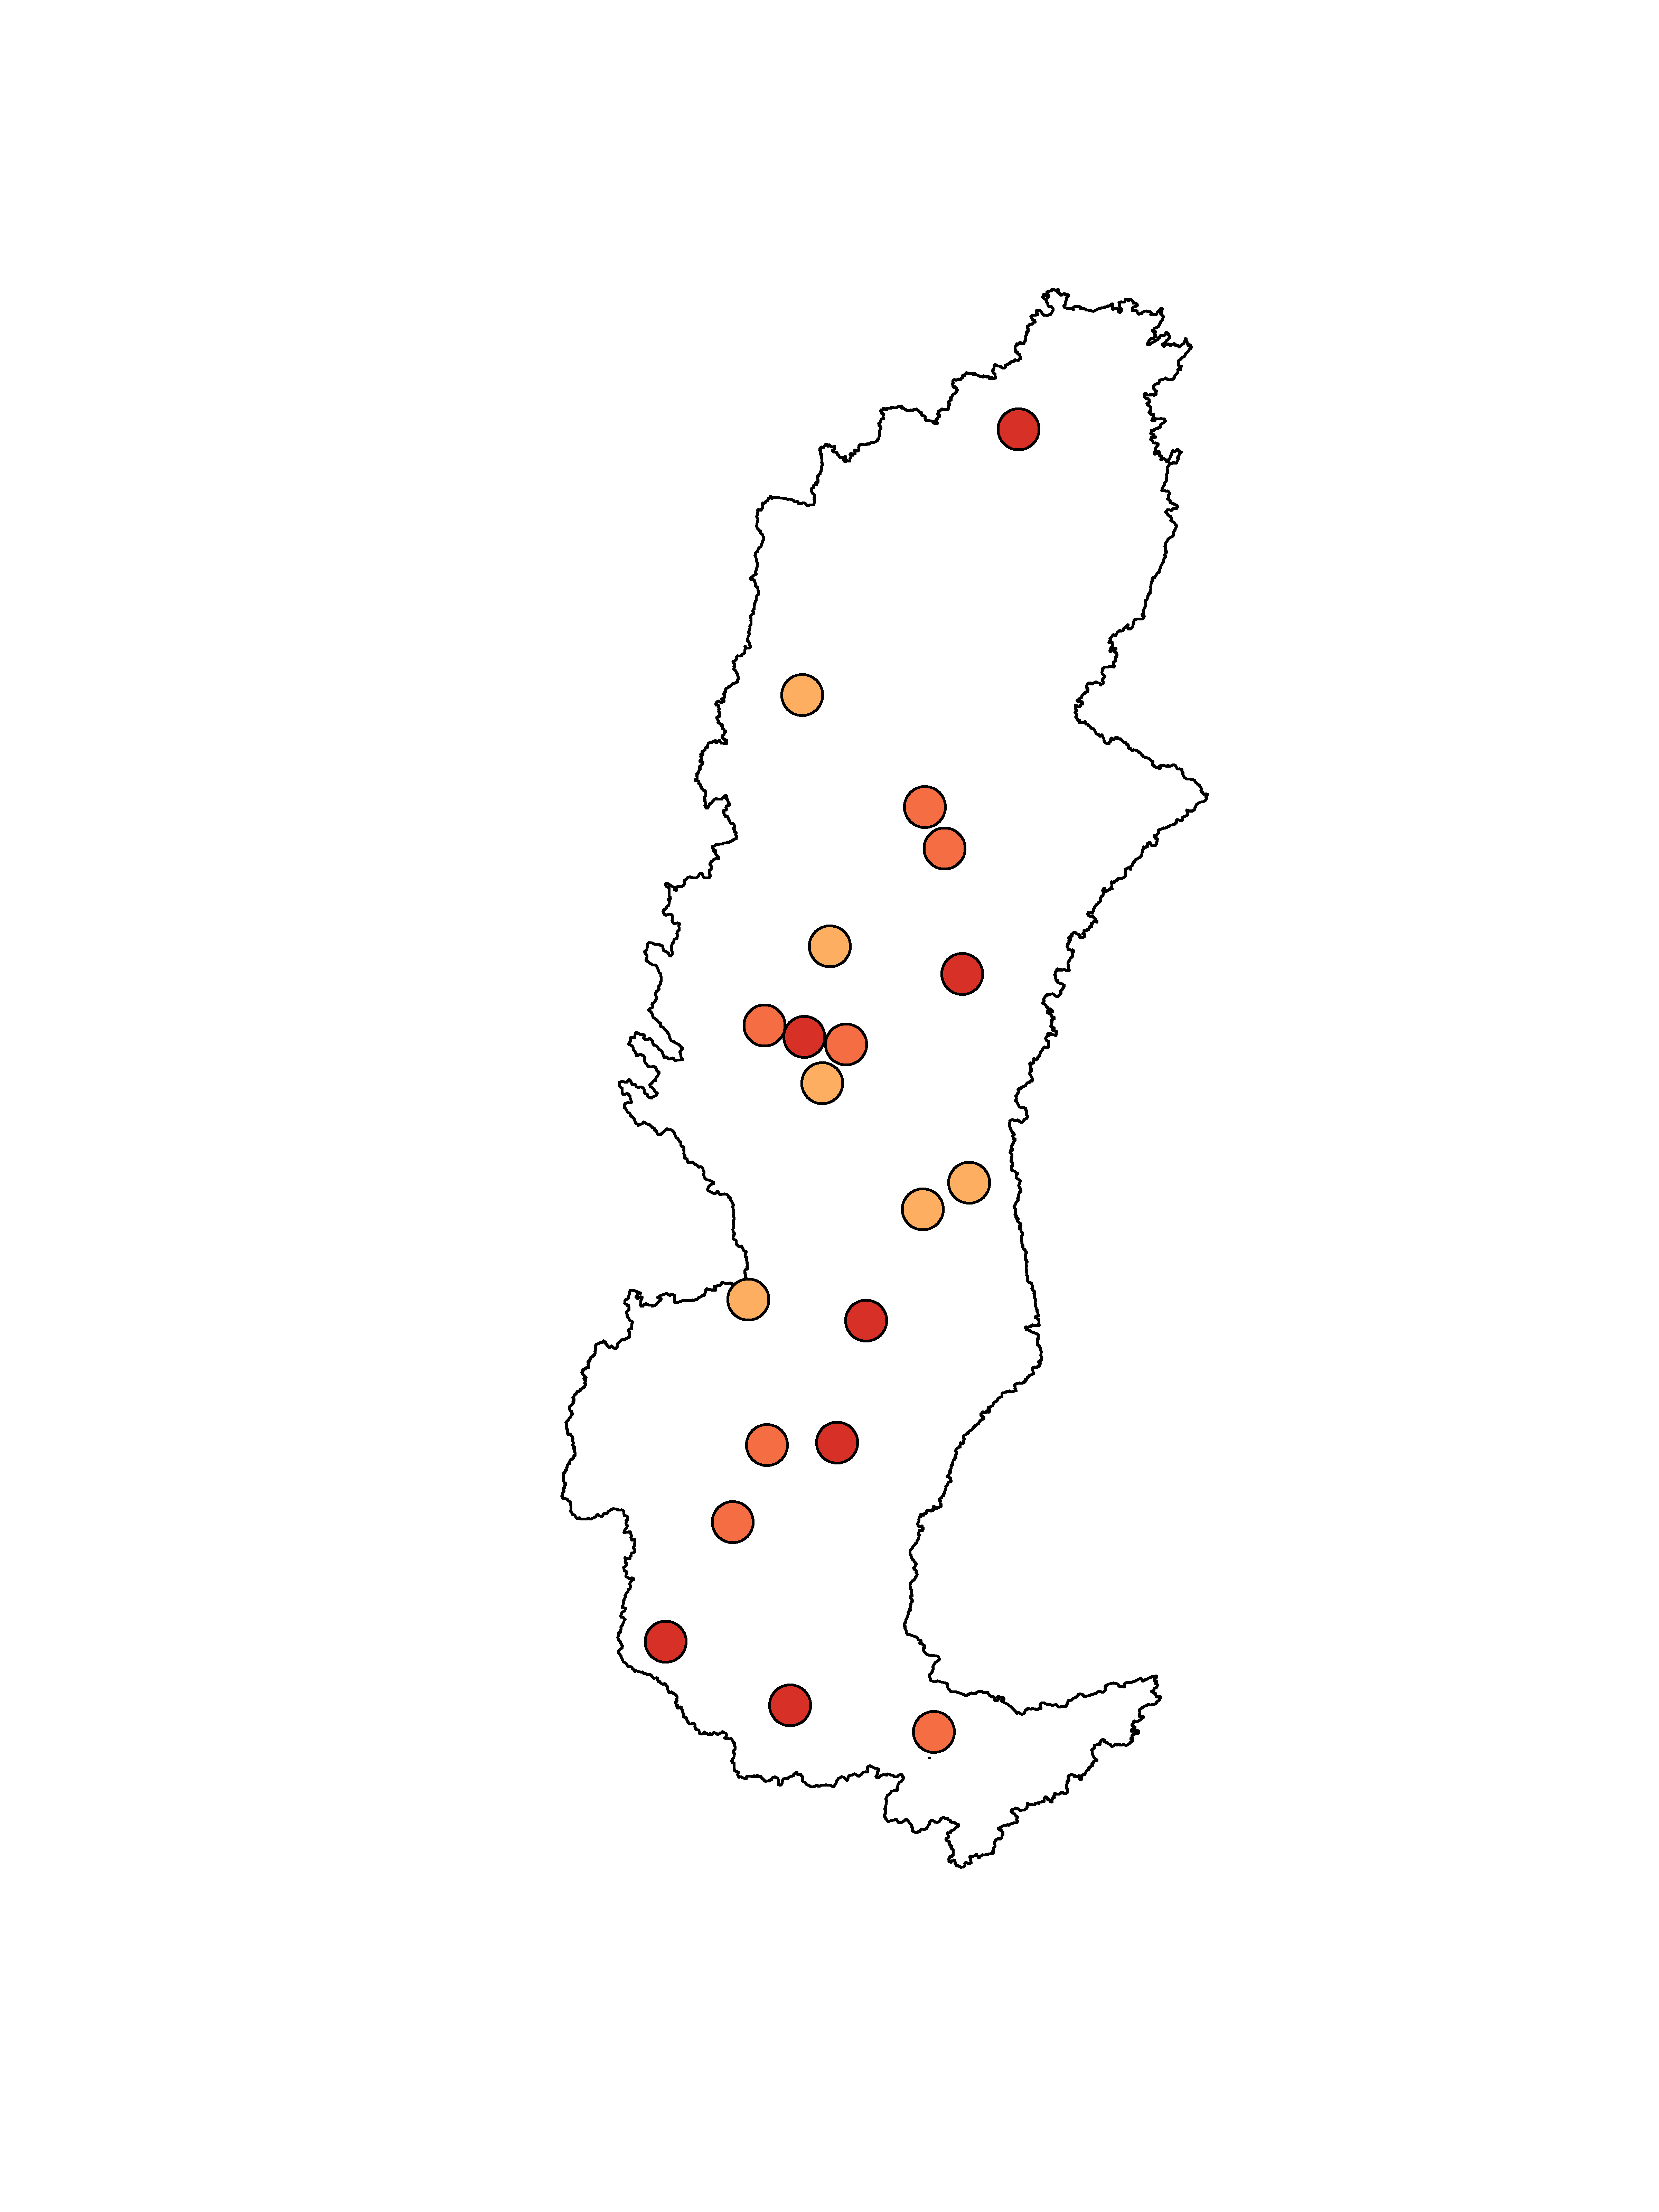
\includegraphics[trim= 4cm 2cm 1cm 2cm, clip, scale = 0.35]{./img/pbias_harg} &
			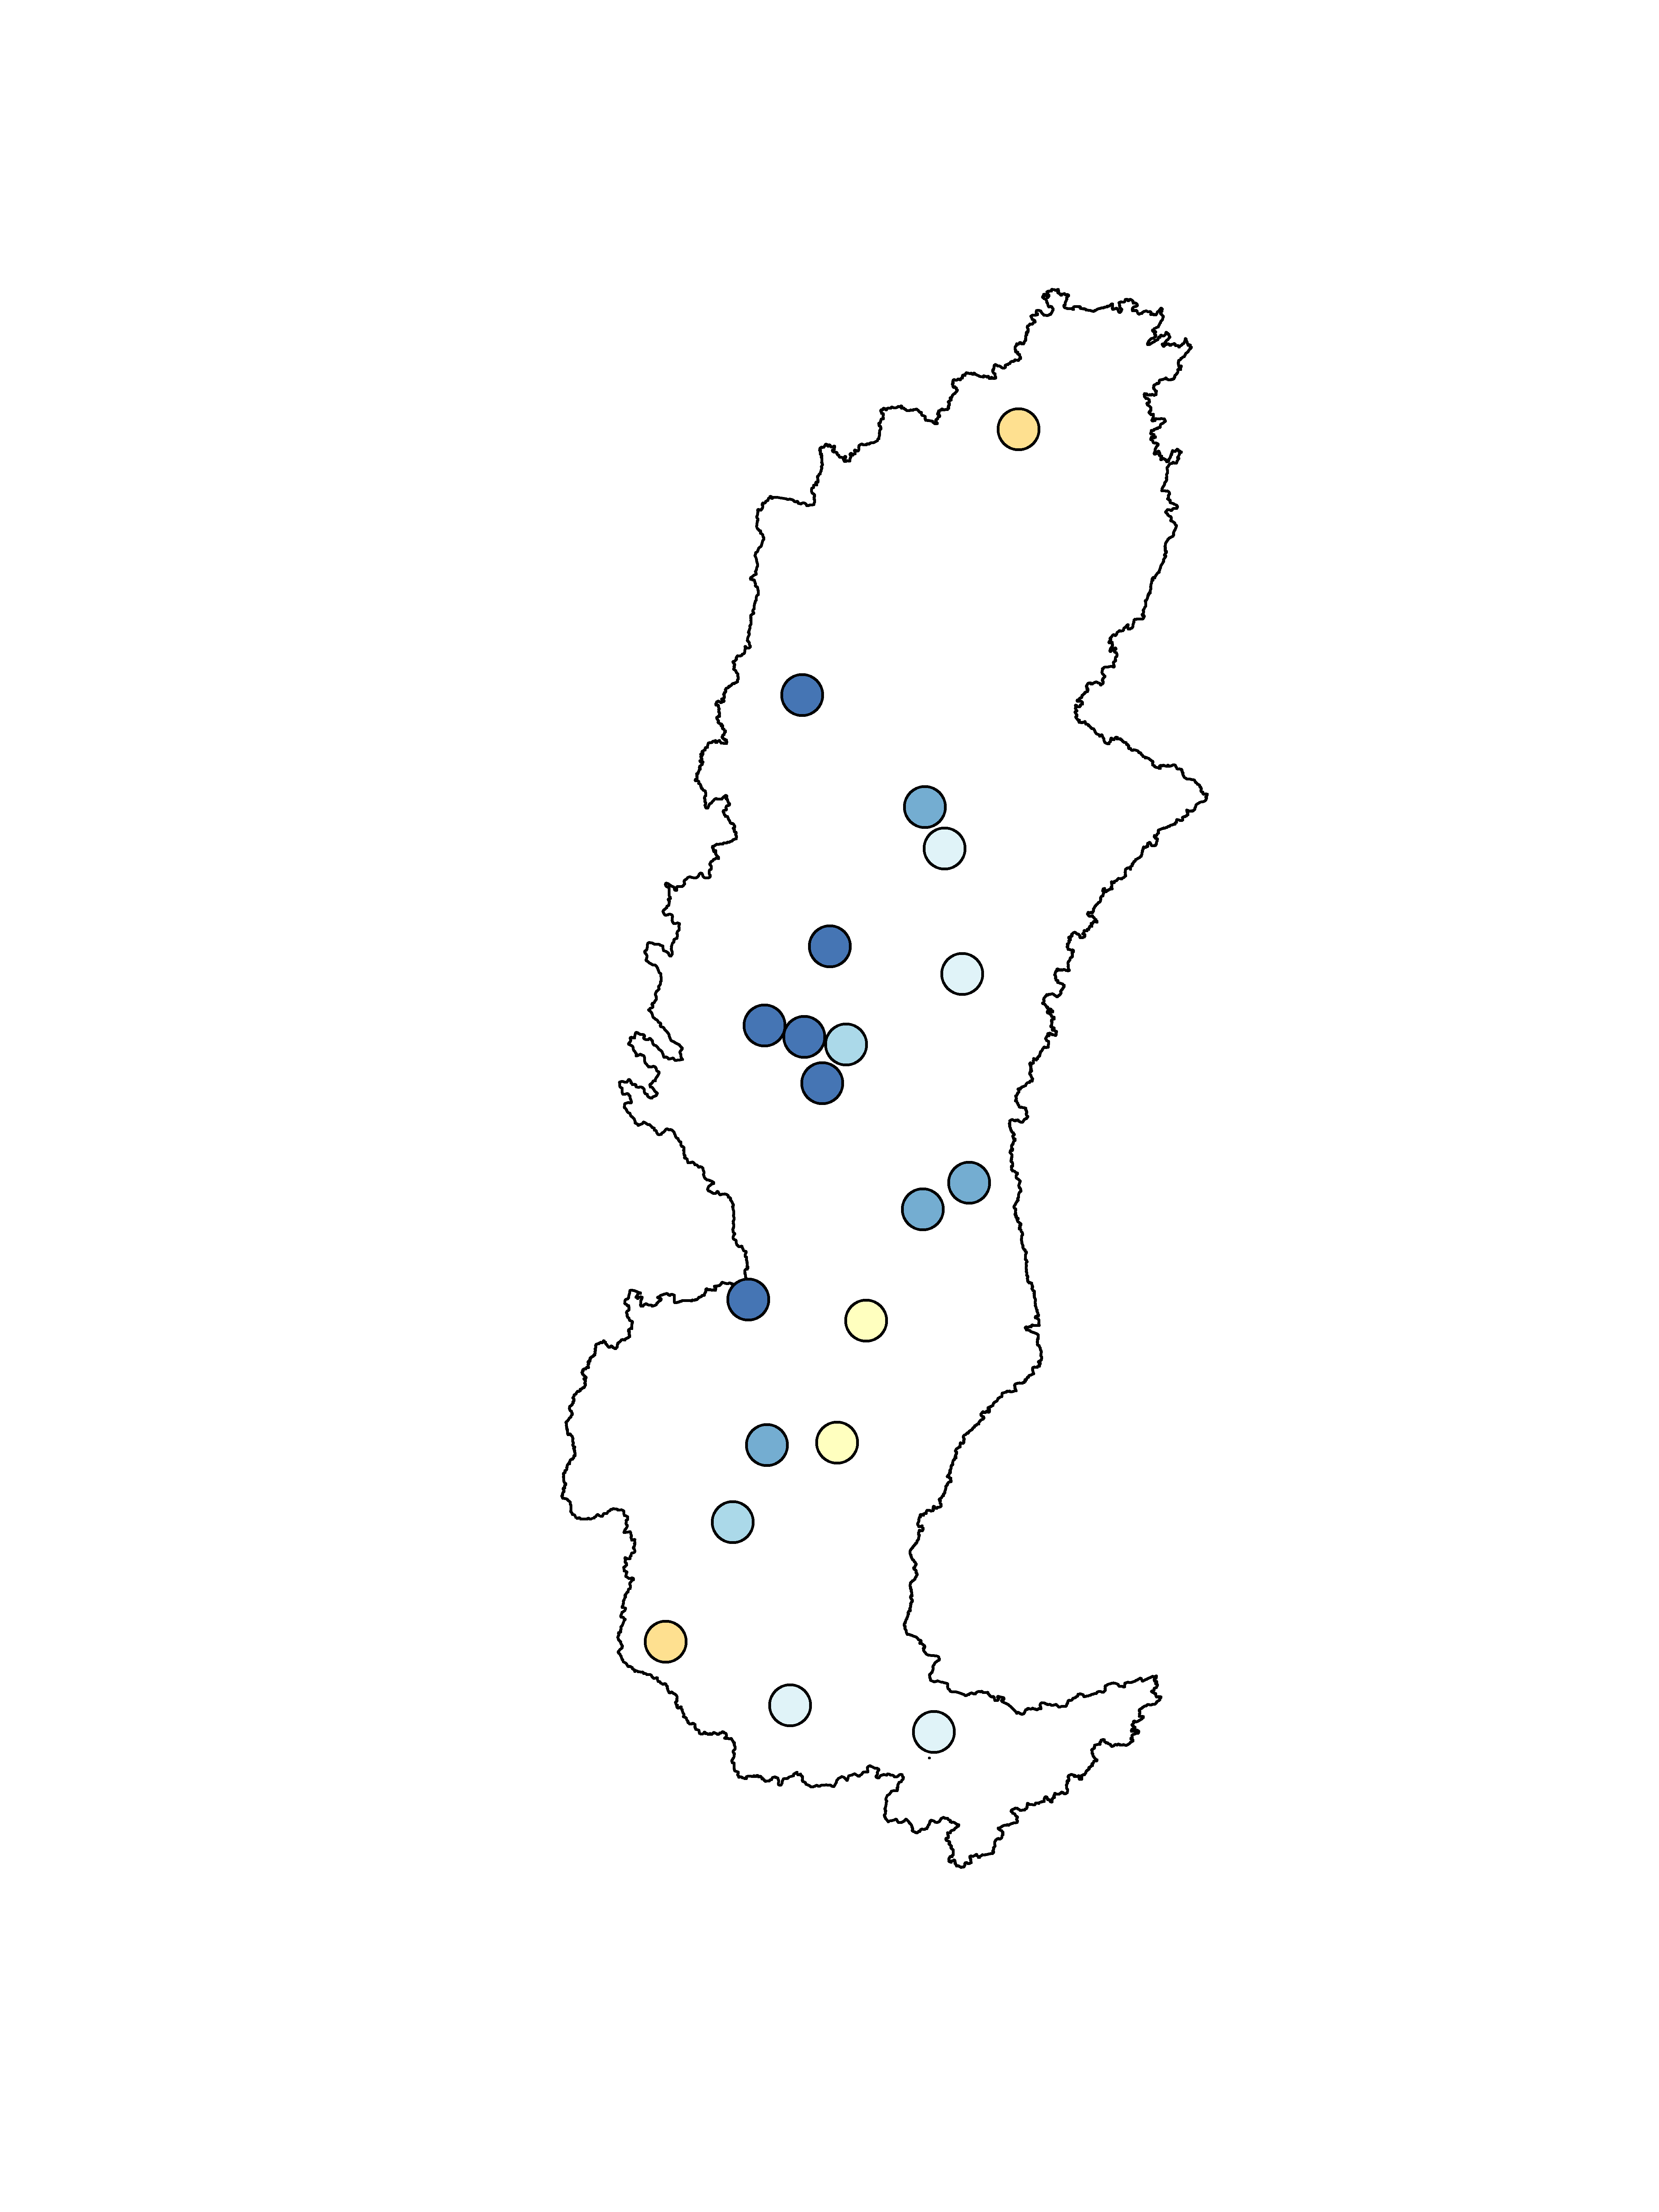
\includegraphics[trim= 4cm 2cm 1cm 2cm, clip, scale = 0.35]{./img/pbias_penman} &
				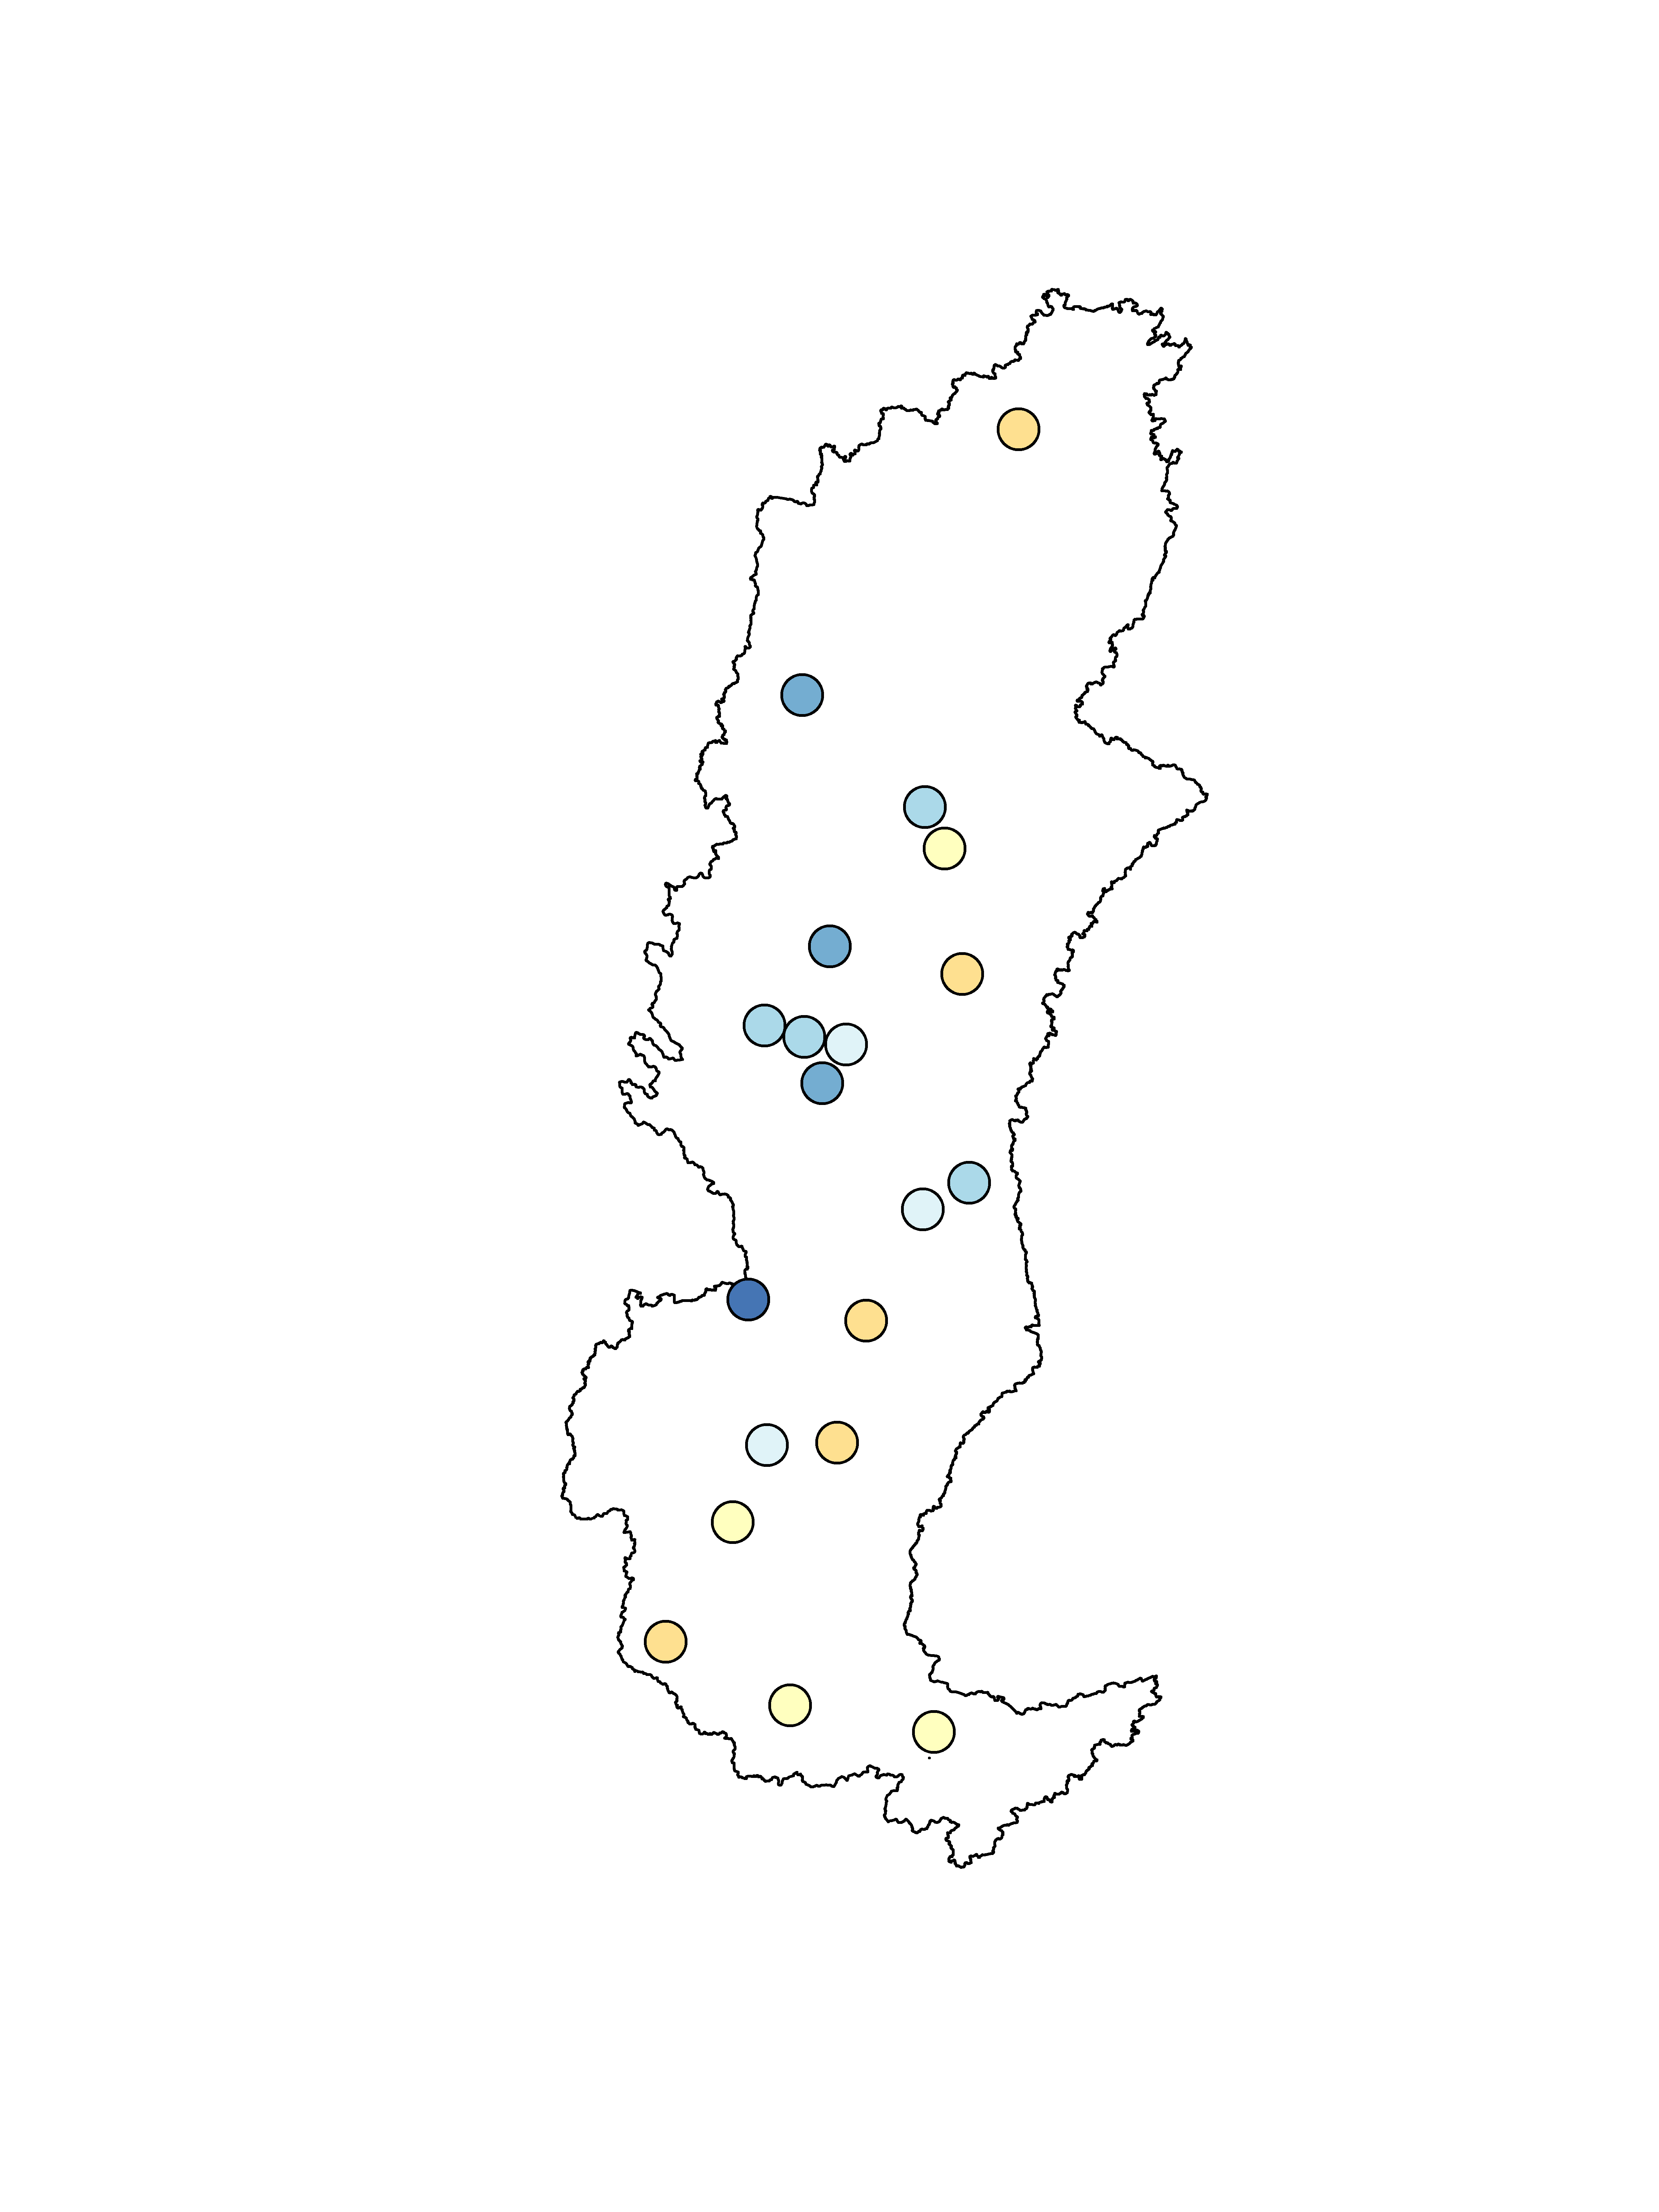
\includegraphics[trim= 4cm 2cm 1cm 2cm, clip, scale = 0.35]{./img/pbias_priestley} &
					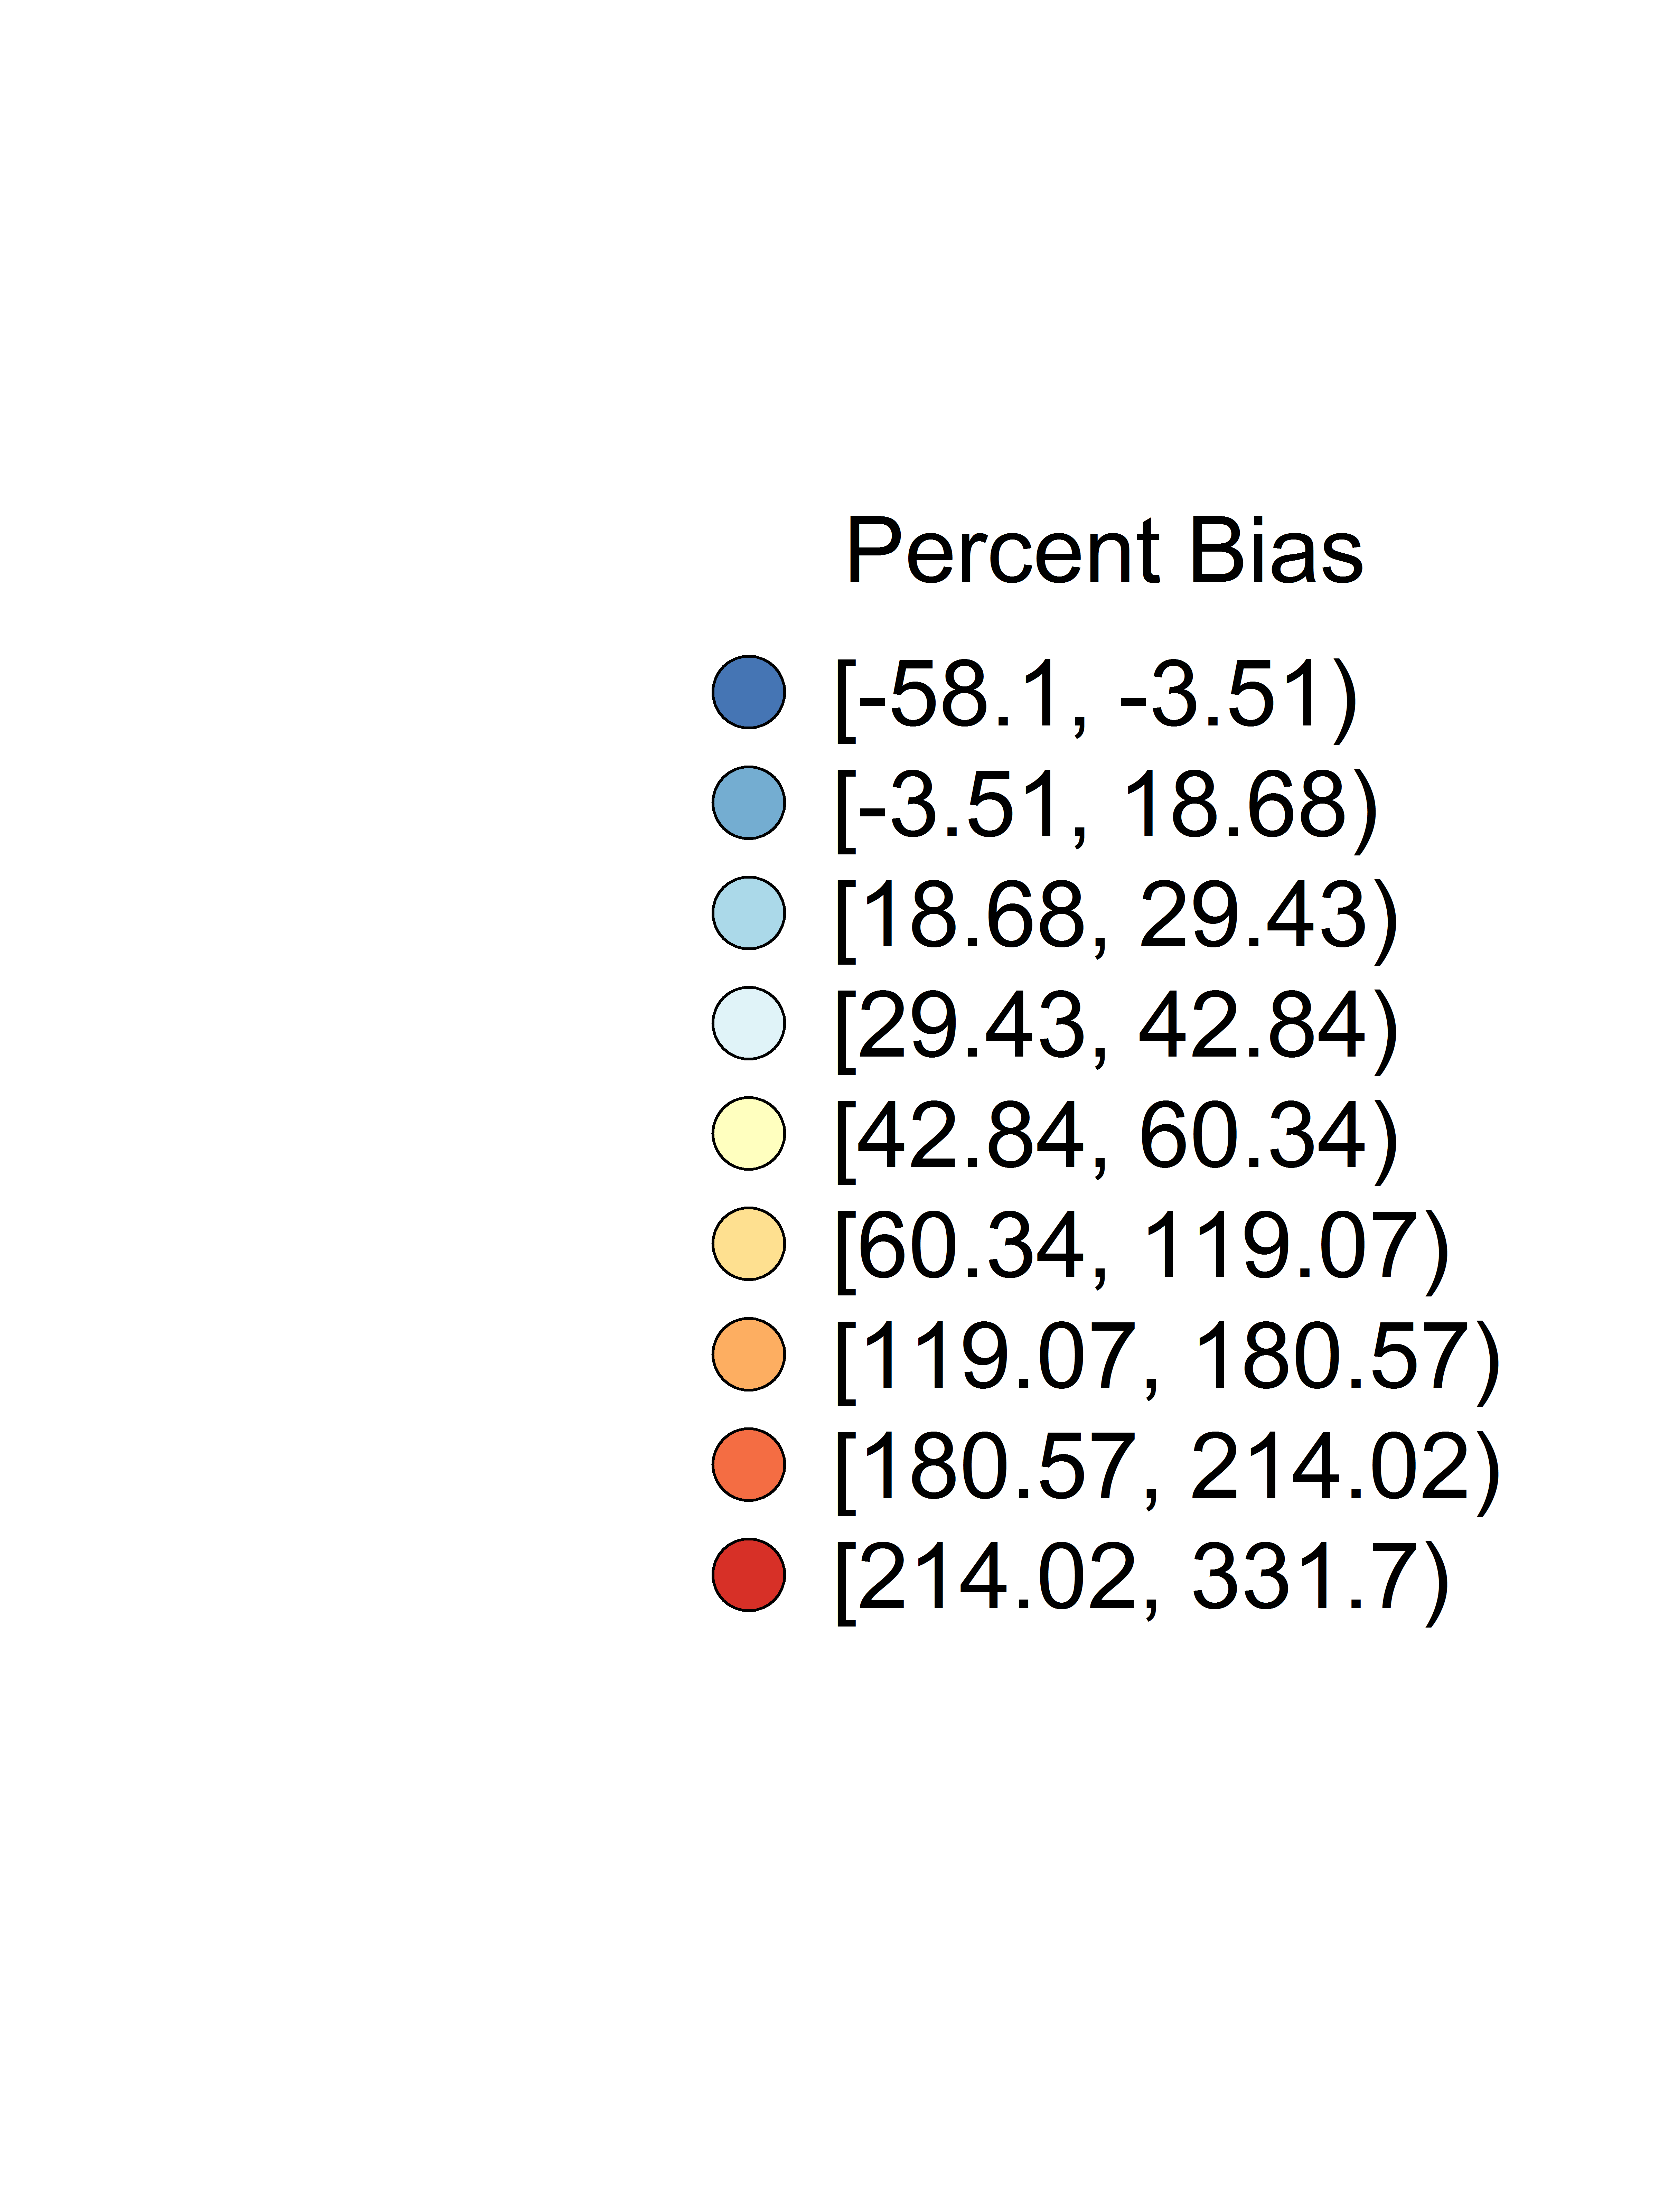
\includegraphics[trim= 5cm 2cm 0cm 3cm, clip, scale = 0.3]{./img/pbias_legend} \\
		{\bf Hargreaves} & {\bf Penman--Monteith} & {\bf Priestely--Taylor} & \\
		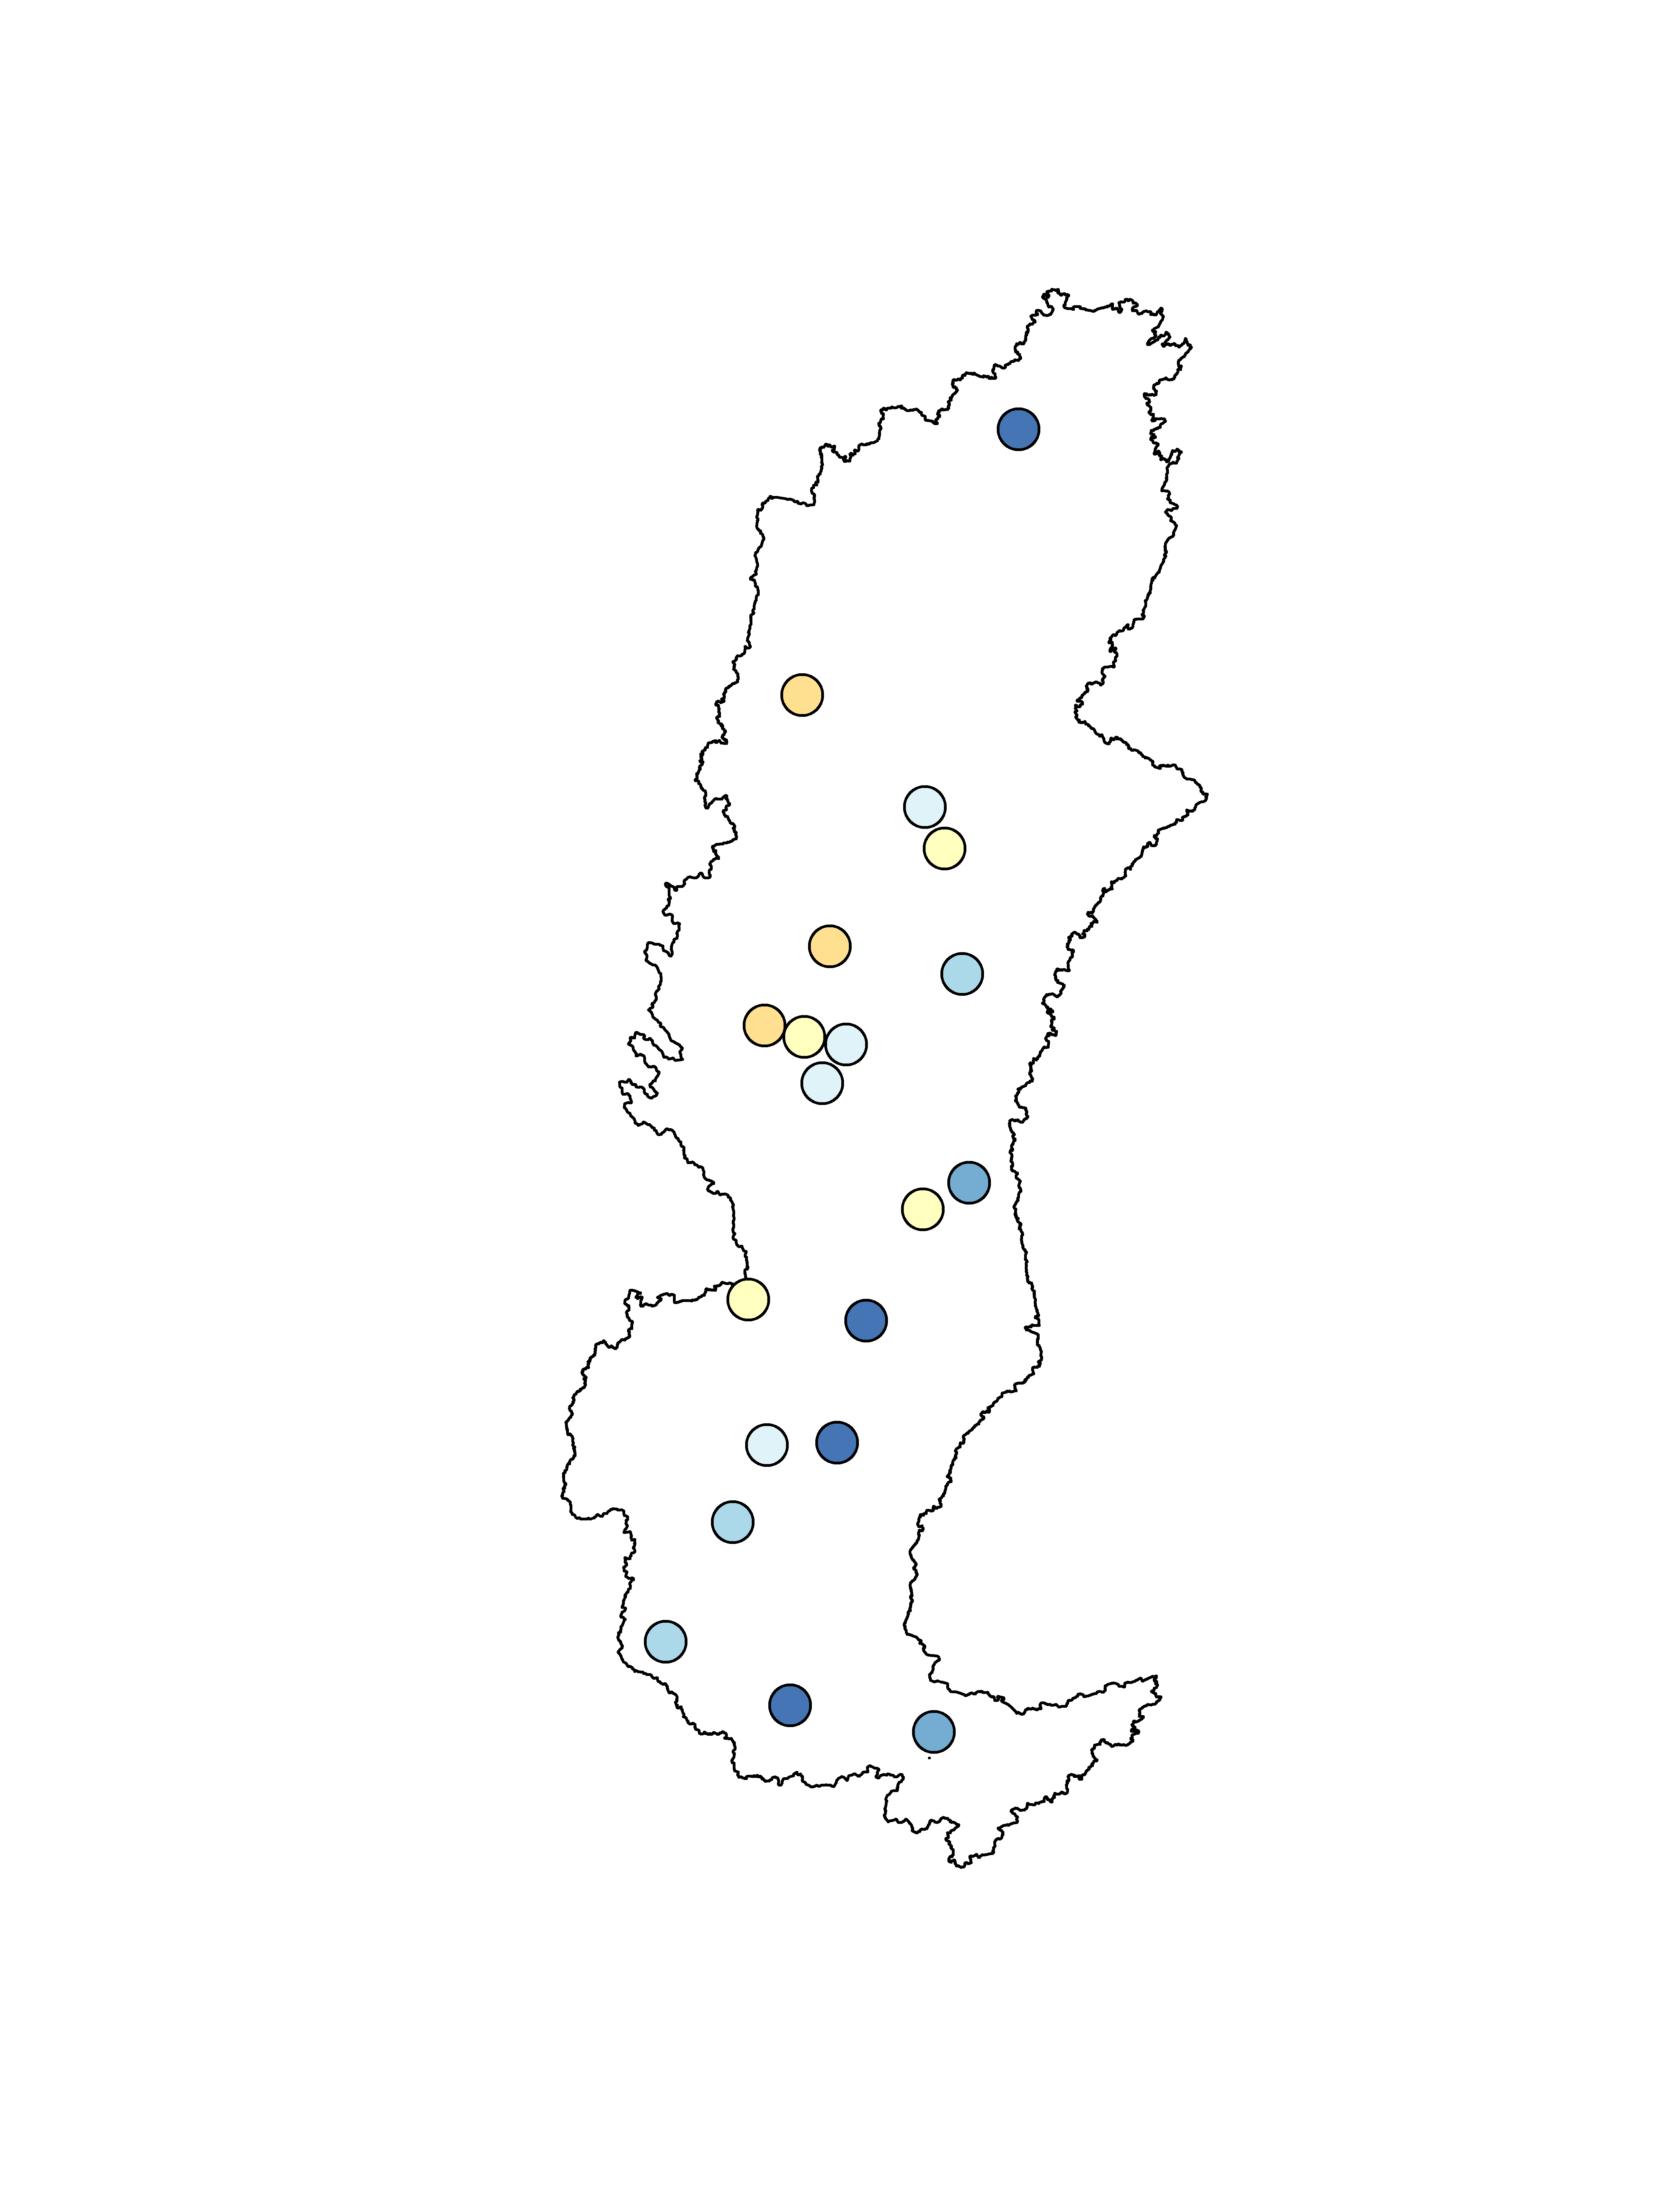
\includegraphics[trim= 4cm 2cm 1cm 2cm, clip, scale = 0.35]{./img/nashsut_harg} &
			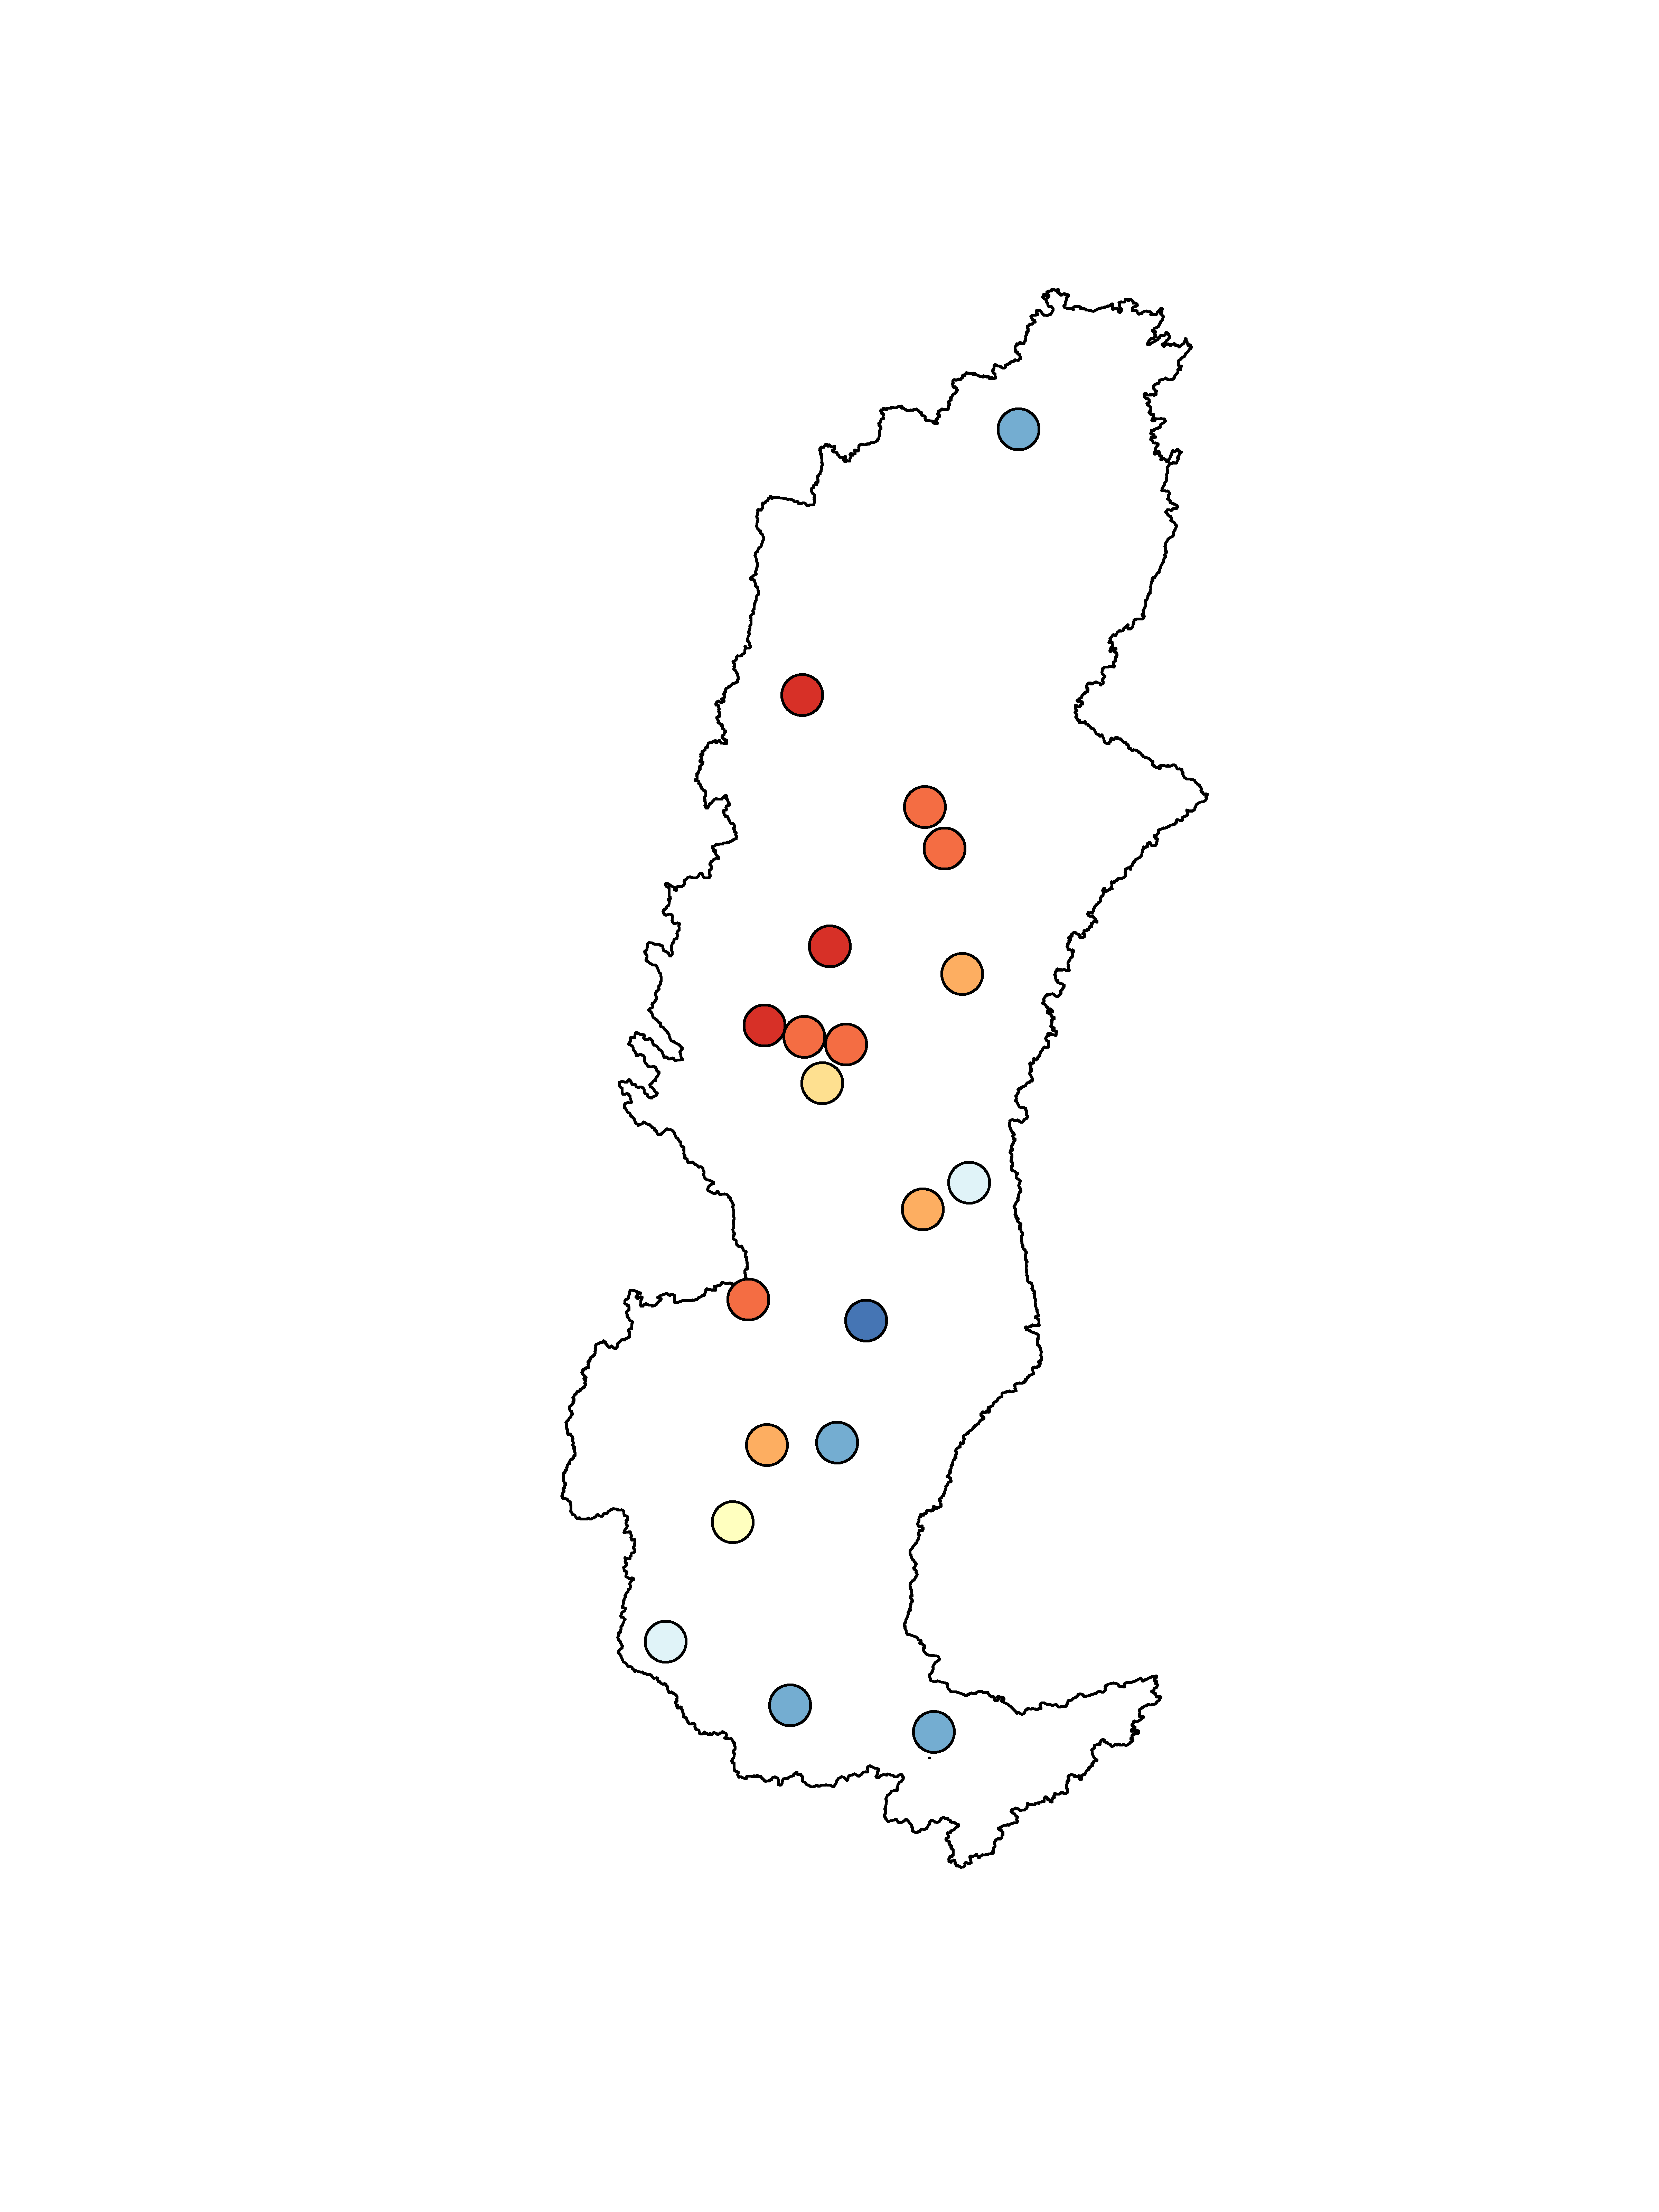
\includegraphics[trim= 4cm 2cm 1cm 2cm, clip, scale = 0.35]{./img/nashsut_penman} &
				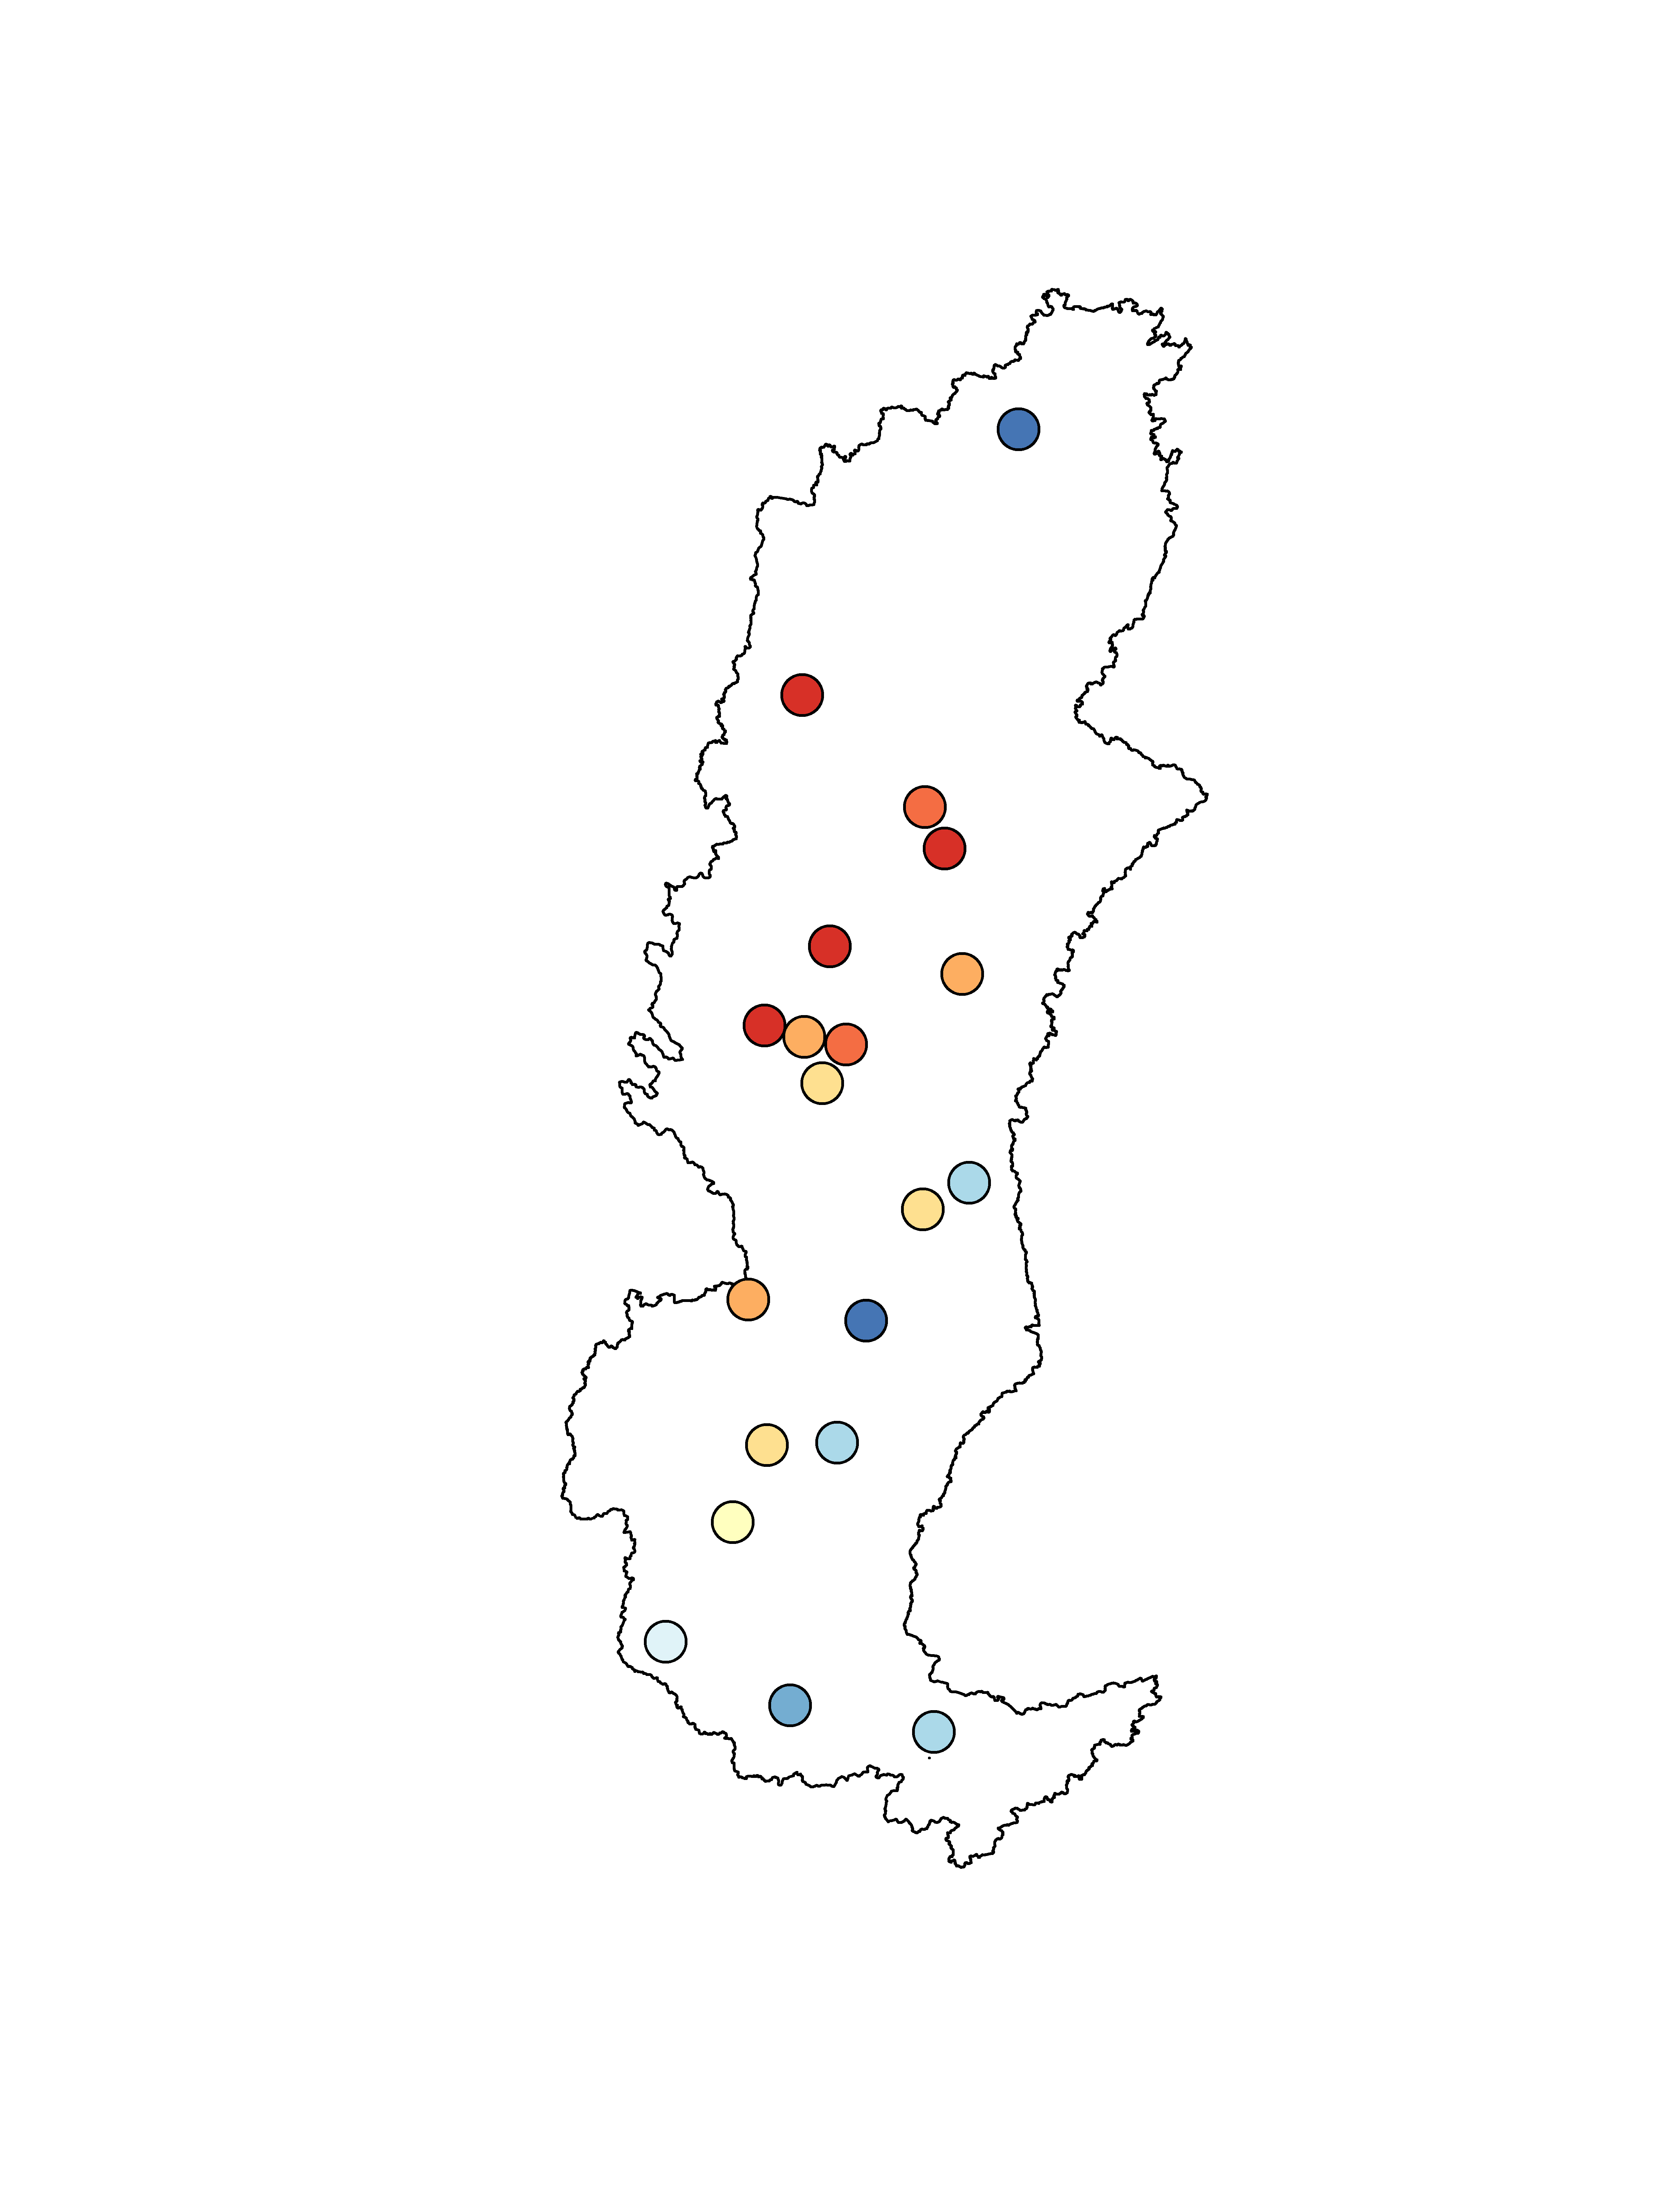
\includegraphics[trim= 4cm 2cm 1cm 2cm, clip, scale = 0.35]{./img/nashsut_priestley} &
					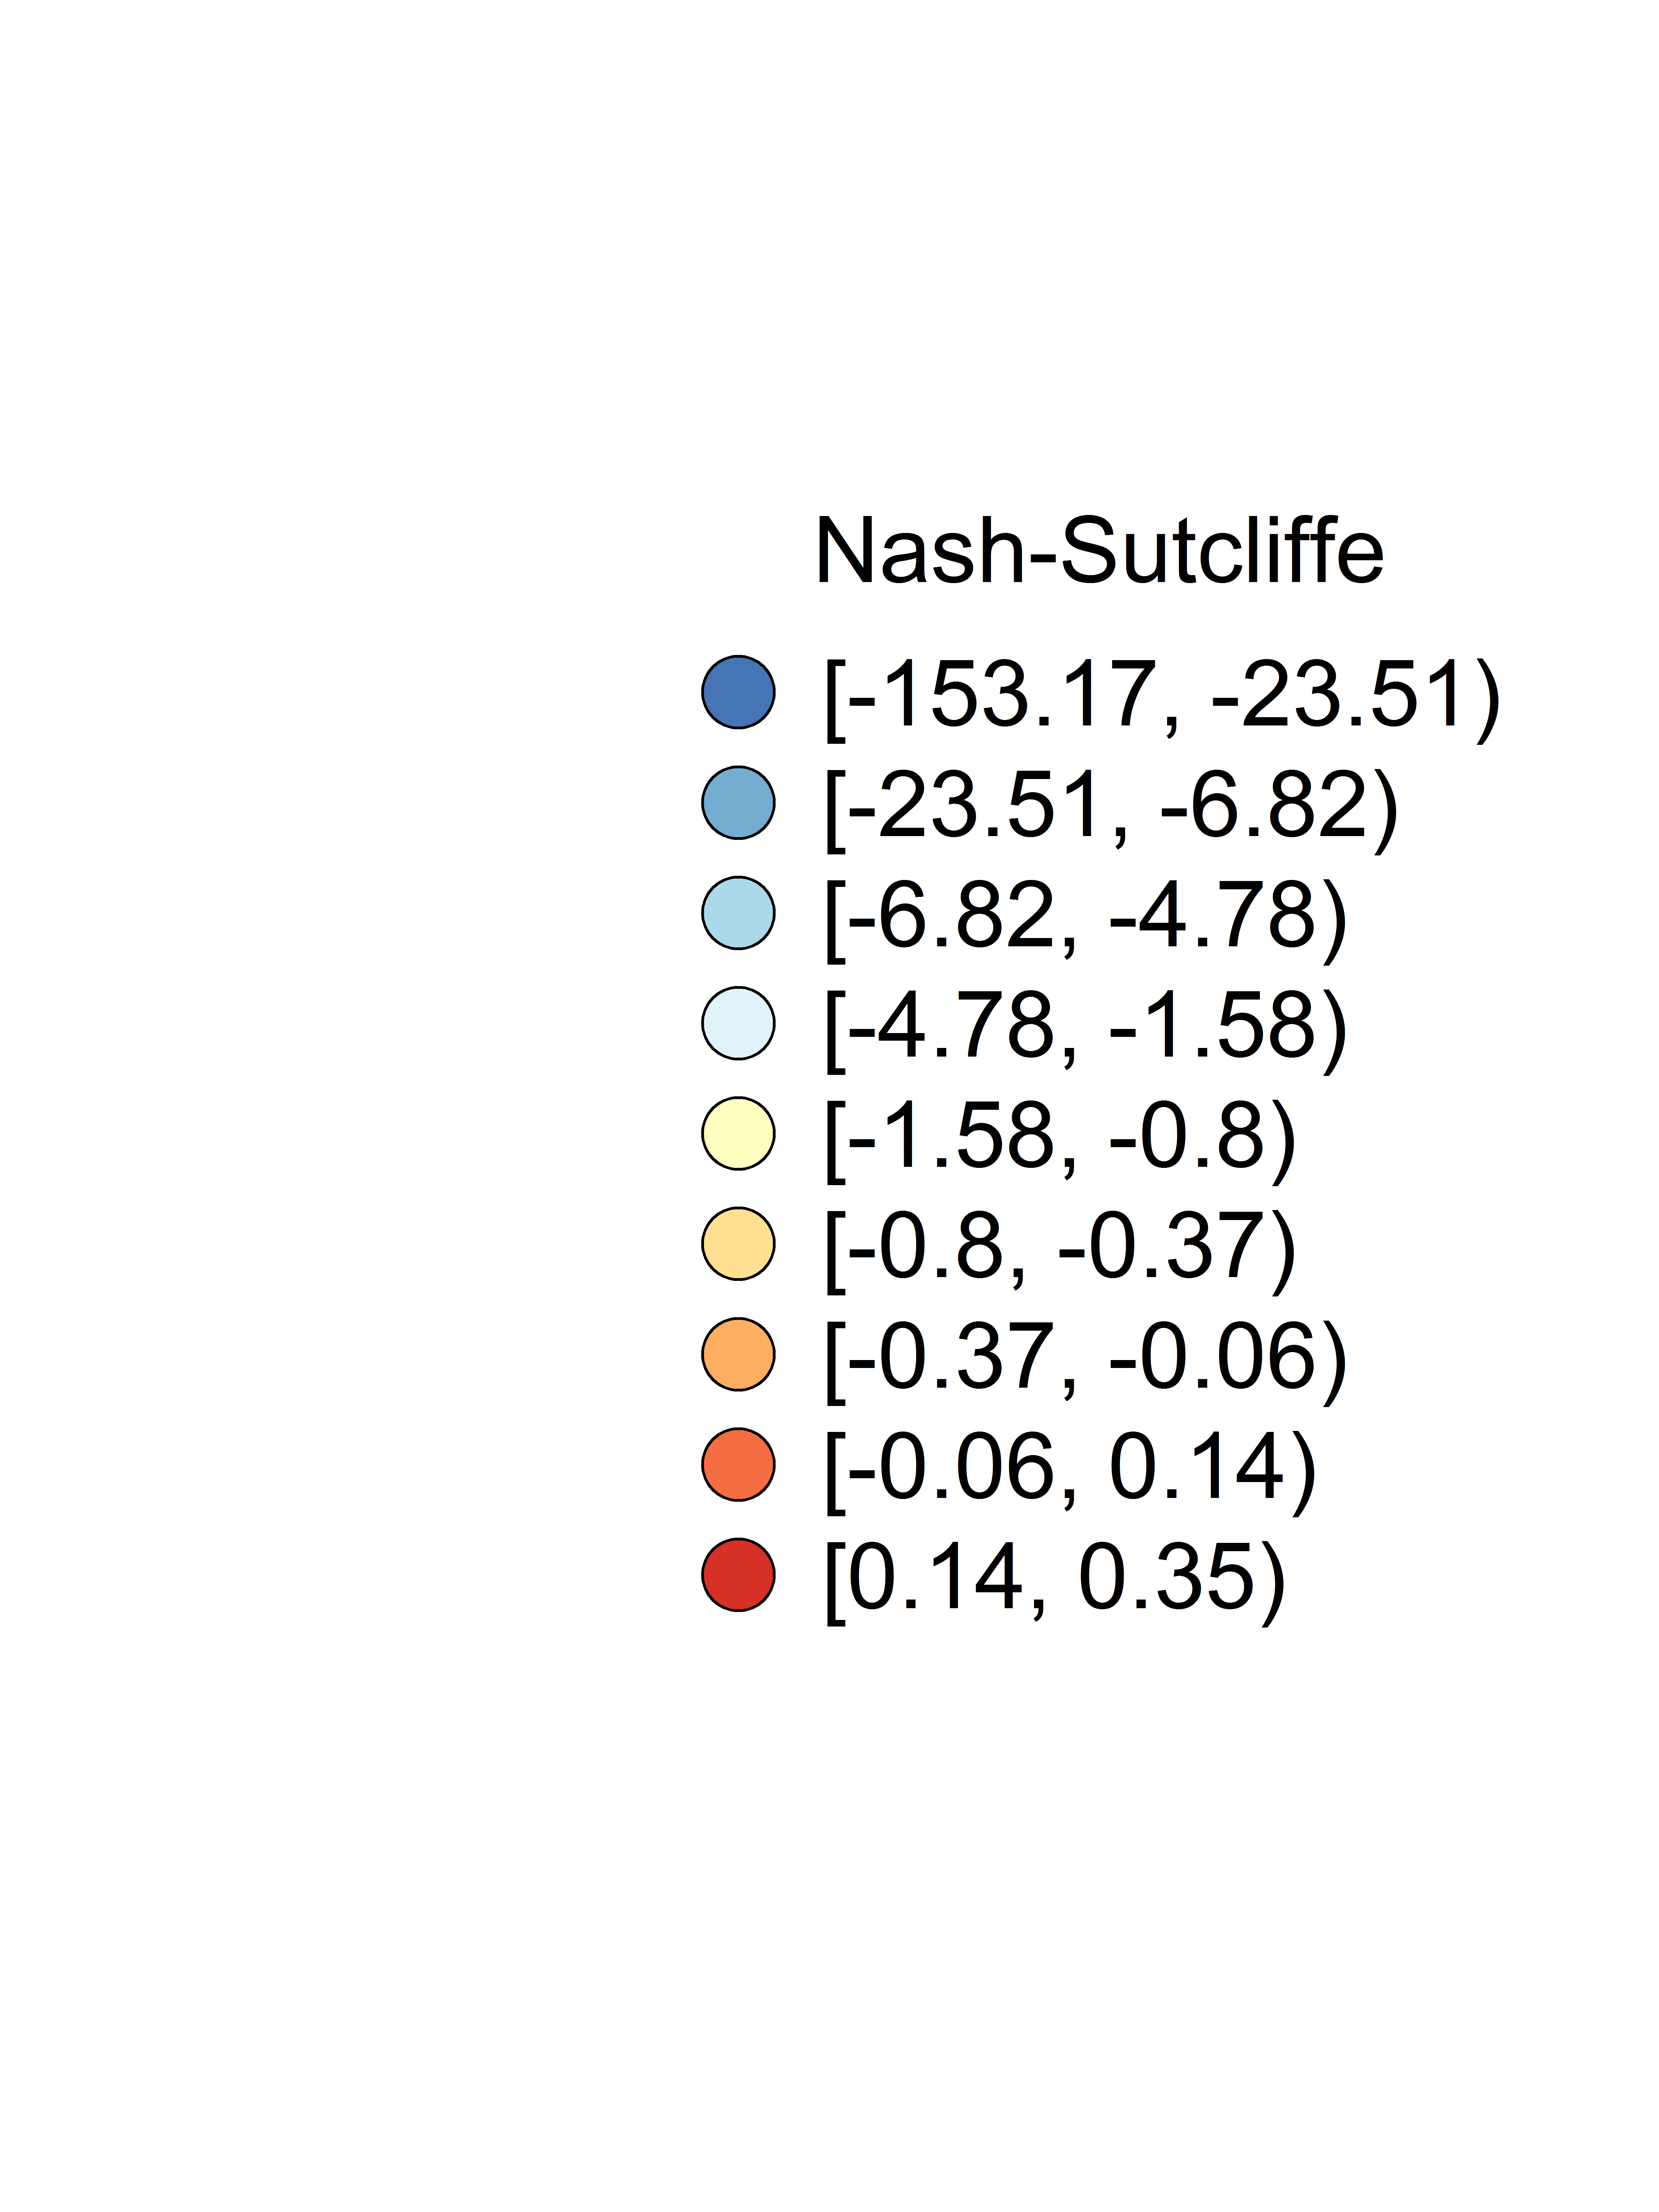
\includegraphics[trim= 5cm 2cm 0cm 3cm, clip, scale = 0.3]{./img/nashsut_legend} \\			
	\end{tabular}
	\caption[Three evapotranspiration methods were examined, Hargreaves]{Three evapotranspiration methods were examined, Hargreaves, Penman--Monteith, and Priestley--Taylor (displayed left to right) each of which was assessed for how well the simulated streamflow matched observed streamflow sites, the value of each is displayed in each map. Each method was assessed using percent bias (top three maps) and the Nash-Sutcliffe model efficiency coefficient (bottom three maps). The Penman--Monteith equation provided the best fit to observed streamflow.}
	\label{fig:et_methods}
\end{figure}
\end{landscape}